%! TEX root = ../../../analisi2.tex

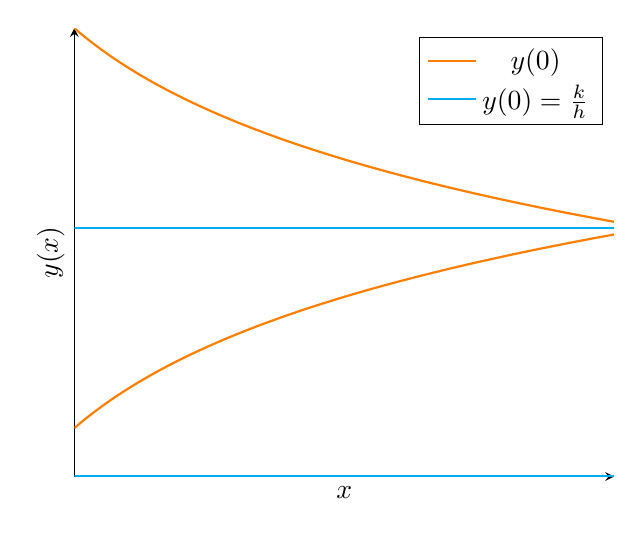
\begin{tikzpicture}
    \begin{axis}[
        axis x line = bottom,
        axis y line = left,
        ylabel = {$y(x)$},
        xlabel = {$x$},
        ticks = none
    ]

        \addplot[
            domain = .2:0.95,
            samples = 100,
            color = orange,
            thick
        ]
        {ln(x) + 2};
        \addlegendentry{$y(0)$}

        \addplot[
            domain = .2:0.95,
            samples = 100,
            color = cyan,
            thick
        ]
        {2};
        \addlegendentry{$y(0) = \frac{k}{h}$}
            
        \addplot[
            domain = .2:0.95,
            samples = 100,
            color = orange,
            thick
        ]
        {2 - ln(x)};

        \addplot[
            domain = .2:0.95,
            samples = 100,
            color = cyan,
            thick
        ]
        {0};
    \end{axis}
\end{tikzpicture}